\chapter{Architektura NFV a VNF} \label{sub:architektura}

V předchozí sekci byla popsána myšlenka a motivace související s virtualizací síťových funkcí. Protože cílem této práce je navržení několika VNF na cloudové platformě, tak je nejprve nutné se seznámit s jeho obecnou architekturou. V této práci se bude vycházet z referenční architektury NVF \cite{NFV_architektura}, která byla navržena organizací ETSI. Jedná se pouze o funkční návrh bez náznaků konkrétní implementace. Od této skupiny existují i podrobnější návrhy jednotlivých částí celého NFV frameworku, které v této práci budou také popsány v příslušných kapitolách.

\begin{figure}[h]
\begin{centering}
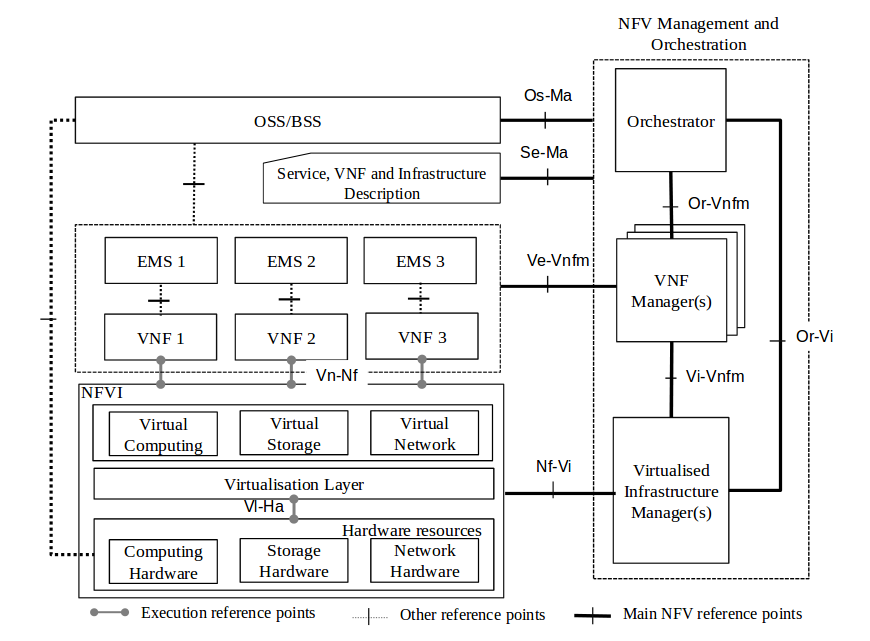
\includegraphics[scale=0.5]{images/NFV_architektura}
\par\end{centering}
\caption{NFV architektura, převzato z \cite{NFV_architektura}\label{fig:NFV_architektura}}
\end{figure}

Jak je vidět na obrázku č. \ref{fig:NFV_architektura}, tak celá architektura se dá rozdělit na tyto 3 hlavní části:

\begin{itemize}
\item Infrastruktura virtualizace síťových funkcí (NFVI) - Jsou všechny softwarové a hardwarové zdroje potřebné k vytvoření prostředí, ve které mohou být jednotlivé VNF být nasazeny. Tato infrastruktura může být velice rozsáhlá, proto je její součástí i síť poskytující konektivitu mezi vzdálenými lokacemi infrastruktury.\cite{NFV_terminology}
\item Virtualizované síťové funkce (VNFs) - Jsou softwarové implementace síťových funkcí, jako je např. NAT a routing. které mohou být nasazeny na NFV infrastruktuře.
\item Management a orchestrace NFV (NFV-MANO) - zde se jedná o řízení softwarových a hardwarových zdrojů v celé infrastruktuře NFV a životního cyklu jednotlivých virtuálních síťových funkcí. Tato část se tedy zaměřuje na řízení a správu všech úloh související v virtualizací v NFV frameworku. \cite{NFV_terminology}
\end{itemize}

Tyto funkční bloky se ještě dále dělí, proto dále v této práci budou tyto jednotlivé části popsány podrobněji a současně k nim budou uvedeny různé možnosti řešení.

\section{Infrastruktura NFV}

Ve zdroji \cite{NFV_infrastructure}, který detailně popisuje infrastrukturu pro virtualizaci síťových funkcí (NFVI), je uvedeno, že je v ní sdružení všech základních zdrojů potřebných pro běh virtuálních síťových funkcí (VNF). Z tohoto důvodu sem patří veškerý hardware. Do NFVI také patří některé softwarové komponenty, které jsou společné mnoho VNF a poskytují funkcionalitu potřebnou pro podporu nasazení, propojení či managementu VNF. Celou infrastrukturu může tvořit jeden či více strojů, které mají tyto potřebné funkce. Tyto stroje také mohou být umístěny v různých spolu spojených lokacích. 

Pro zjednodušení lze celou NFV infrastrukturu rozdělit do 3 následujících domén:

\begin{itemize}
\item Compute Domain - Do této domény patří veškeré hardwarové zdroje jako jsou servery, úložiště a komponenty, které tyto zdroje obsahují, např. procesory, pevné disky, síťové karty, atd. Zároveň je zde řešen návrh fyzické topologie. \cite{NFV_compute}
\item Hypervisor Domain - Toto je doména, které představuje softwarové prostředí abstrahující hardware v compute doméně a poskytuje je jako virtuální zdroje. Tyto zdroje následně mohou využívat virtuální síťové funkce. \cite{NFV_hypervisor}
\item Infrastructure Network Domain - V této doméně je řešeno veškeré propojení výše zmíněných domén. Tedy fyzické i virtuální infrastruktury.\cite{NFV_network}
\end{itemize}

Funkci obsaženou v jednotlivých doménách znázorňuje obrázek č. \ref{fig:infrastruktura}. Více informací na tuto problematiku lze nalézt v \cite{NFV_infrastructure} a ve zdrojích uvedených u každé domény. 

\begin{figure}[h]
\begin{centering}
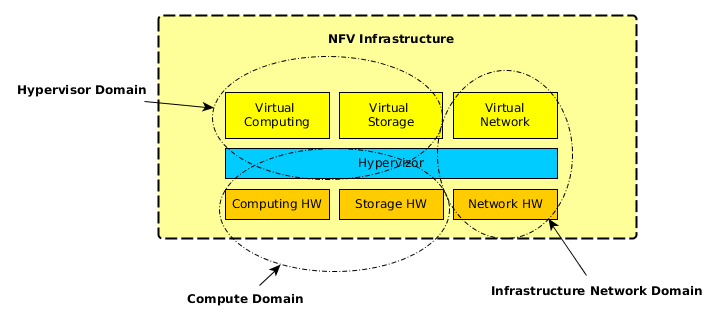
\includegraphics[scale=0.65]{images/infrastruktura}
\par\end{centering}
\caption{Schéma NFV infrastruktury\label{fig:infrastruktura}}
\end{figure}

Dá se říci, že referenční návrh infrastruktury pro NVF je podobný jako pro návrh infrastruktury pro cloud computing platformu. Měl by se tedy skládat z generických a komerčně vysoce dostupných serverů, které by měli být zapojeny do switche a tím by měla být zajištěna konektivita. Na tyto servery je následně nasazen jeden z dostupných hypervisorů. Výběr správného hypervisoru, které jsou v současné době dostupné na trhu, je hlavní podmínka správného a funkčního návrhu této části NFV frameworku. Přehled hypervisorů je uveden v kapitole \ref{sub:Hypervisor}. V produkčním prostředí by součástí řešení bylo samozřejmě řešení síťového návrhu. Tato práce však má sloužit pouze jako ukázka a z tohoto důvodu zde nebude síťový návrh zmíněn.

\section{Virtuální síťová funkce}

Virtuální síťová funkce (VNF) je dle \cite{NFV_VNF} určitá síťová funkce, která běží na NVF infrastruktuře a je zároveň NVF frameworkem řízena a spravována. Zároveň musí mít dobře definované rozhraní k ostatním síťovým funkcím, k VNF Managerovi a měla by obsahovat management rozhraní či port. Jedna VNF může být být obsažena v jednom virtuálním stroji nebo může být roztažena přes více virtuálních strojů. 

Na obrázku č. \ref{fig:VNF} je vidět jednoduché schéma virtuální síťové funkce dle referenčního návrhu \cite{NFV_VNF}. Celý životní cyklus VNF, což je vytvoření, spuštění, zastavení, smazání a škálování, řídí VNF Manager, který je součástí NVF managementu a orchestrace. Současně je možné dynamicky změnit aktuální konfiguraci pomocí Entity manageru (EM) přes management interface. EM může spravovat více VNF nebo právě jednu. Vnitřní struktura celé instance může být tvořena více komponentami (VNFC), které spolu mohou být navzájem provázány. Toto provázání však nemusí být viditelné zvenčí.

\begin{figure}[h]
\begin{centering}
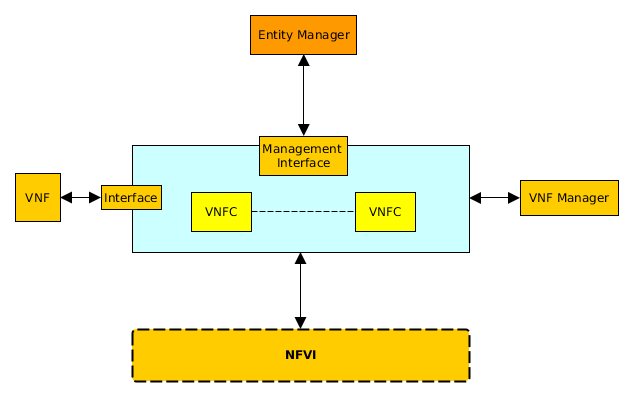
\includegraphics[scale=0.67]{images/VNF}
\par\end{centering}
\caption{Schéma virtuální síťové funkce\label{fig:VNF}}
\end{figure}

Pohledem na současný trh zjistíme, že VNF je prakticky poskytována ve 3 základních podobách.

\begin{itemize}
\item Softwarová aplikace - V tomto případě je poskytována VNF jako aplikace, která může být nainstalována na běžný operační systém jako je například GNU/Linux.
\item Ucelený operační systém - Zde je poskytován přímo celý operační systém, který může být nainstalován do virtuálního stroje nebo i na fyzický server.
\item Kompletní VM - Poskytovatel VNF může dát k dispozici rovnou přetvořený obraz virtuálního stroje (image), který může obsahovat operační systém se síťovými funkcemi. Tento systém však nemusí být klasicky dostupný operační systém jako je GNU/Linux či FreeBSD, ale může se jednat o speciálně vytvořený systém od výrobce. Tento způsob budou využívat poskytovatelé, kteří mají proprietární řešení pro síťová řešení jako je například Cisco či Juniper.
\end{itemize}

\section{Management a orchestrace NFV}

Management a orchestrace virtualizace síťových funkcí (NFV MANO) je nejdůležitější část celého NFV frameworku. Je tomu tak, protože MANO zajišťuje správné fungování NFV infrastruktury i jednotlivých virtuálních síťových funkcí. MANO také poskytuje funkce nutné pro provisioning VNF a související operace, jako je jejich konfigurace jednotlivých VNF a infrastruktury, na které běží. Zároveň spravuje a řídí životní cyklus fyzických a virtuálních zdrojů, které slouží pro podporu VNF. 

\begin{figure}[h]
\begin{centering}
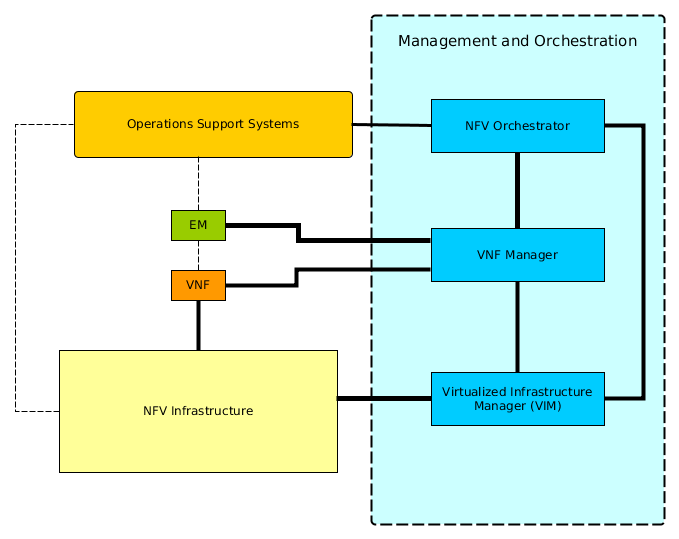
\includegraphics[scale=0.65]{images/MANO}
\par\end{centering}
\caption{Schéma NFV MANO\label{fig:MANO}}
\end{figure}

Jak vyplývá z obrázku č. \ref{fig:MANO}, tak referenční návrh MANO dle \cite{NFV_MANO} se skládá ze hlavních 3 částí, které se zabývají správnou jednotlivých vrstev NFV frameworku.

\begin{itemize}

\item Virtualized infrastructure manager (VIM) - Řídí a spravuje fyzické a virtuální zdroje v jedné doméně infrastuktury. Celková infrastruktura se může skládat z více domén a každá musí mít svůj VIM. Jeho typickými úlohami jsou vytvýření, udržování a uvolňování VM na dostupných zdrojích v doméně. Zároveň musí mít přehled o všech těchto a stavu hardwarových zdrojů.

\item VNF manager - Dohlíží na lifecycle management jednotlivých VNF instancí. To znamená, že výtváří, udržuke a ukončuje VNF instance, které běží na jednotlivých VM (ty však spravuje VIM). Opět může existovat více VNF managerů, kteří mohou spravovat jednu či více VNF.

\item NFV orchestator - Zjednodušeně slouží jako řízení a správu všech VIM a všech VNF managerů. Pomocí komunikace s VIM dokáže spravovat dostupné zdroje a pomocí komunikace s VNF managery dokáže řídit síťové služby. Jeho další funkcí je i přehled všech dostupných VNF, neboli katalog VNF, a registrace nových VNF do tohoto katalogu. Ten je pak dostupný uživatelům.
\end{itemize}

Celý systém je navržen tak, že by měl pracovat společně se stávajícími aplikacemi a systémy, které potencionální uživatelé používají pro provoz své infrastruktury a podnikových procesů (Operation support system).

V oblasti NFV MANO probíhá v součastnosti rozsáhlí vývoj a existuje několik projektů, které se tím zabývají. V článek \cite{NFV_orchestration} je nabídnut zajímavý přehled.






